\ChapterImageStar[cap:dar]{Análisis de Decisiones y Resolución}{./images/fondo.png}\label{cap:dar}
\mbox{}\\
\section{Metodología de evaluación}
\noindent
La metodología de evaluación que se aplicó para la elección de la tecnología de \VBC fue \textit{Decision, analysis and resolution} (\DAR) de CMMI \citep{CMMIInstitute2010}. Esta metodología permitió evaluar las necesidades del grupo \GRID\ a través de un proceso estructurado que consideró múltiples alternativas, criterios de evaluación bien definidos y un análisis comparativo. En este caso, se analizaron las tecnologías \VBC\ encontradas en la revisión literaria, aplicando criterios como el tipo de licencia, la compatibilidad con herramientas de orquestación, el rendimiento entre otros. Así, el uso de \DAR\ no solo busca aportar transparencia al proceso, sino también trazabilidad y justificación técnica frente a una decisión para la arquitectura de infraestructura basada en contenedores.
El proceso de evaluación quedó registrado en un vídeo explicativo disponible en \href{https://youtu.be/xOmuQs2RX2c}{link}.

\section{Resultados de la evaluación}
\noindent
La tabla~\ref{tab:tabla-dar} presenta la aplicación de la metodología \DAR\ al proceso de selección de tecnologías de \VBC\. Este enfoque permitió evaluar de manera estructurada diversos criterios como el tipo de licencia, compatibilidad con orquestadores, soporte para redes y volúmenes, documentación disponible, consumo de recursos y costo de implementación en entornos productivos. Al asignar valores ponderados a cada aspecto, el análisis facilita la comparación objetiva entre múltiples alternativas, proporcionando un marco de referencia sólido para identificar la solución más adecuada según las necesidades técnicas, operativas y estratégicas de un proyecto.
\begin{table}[H]
    \centering
    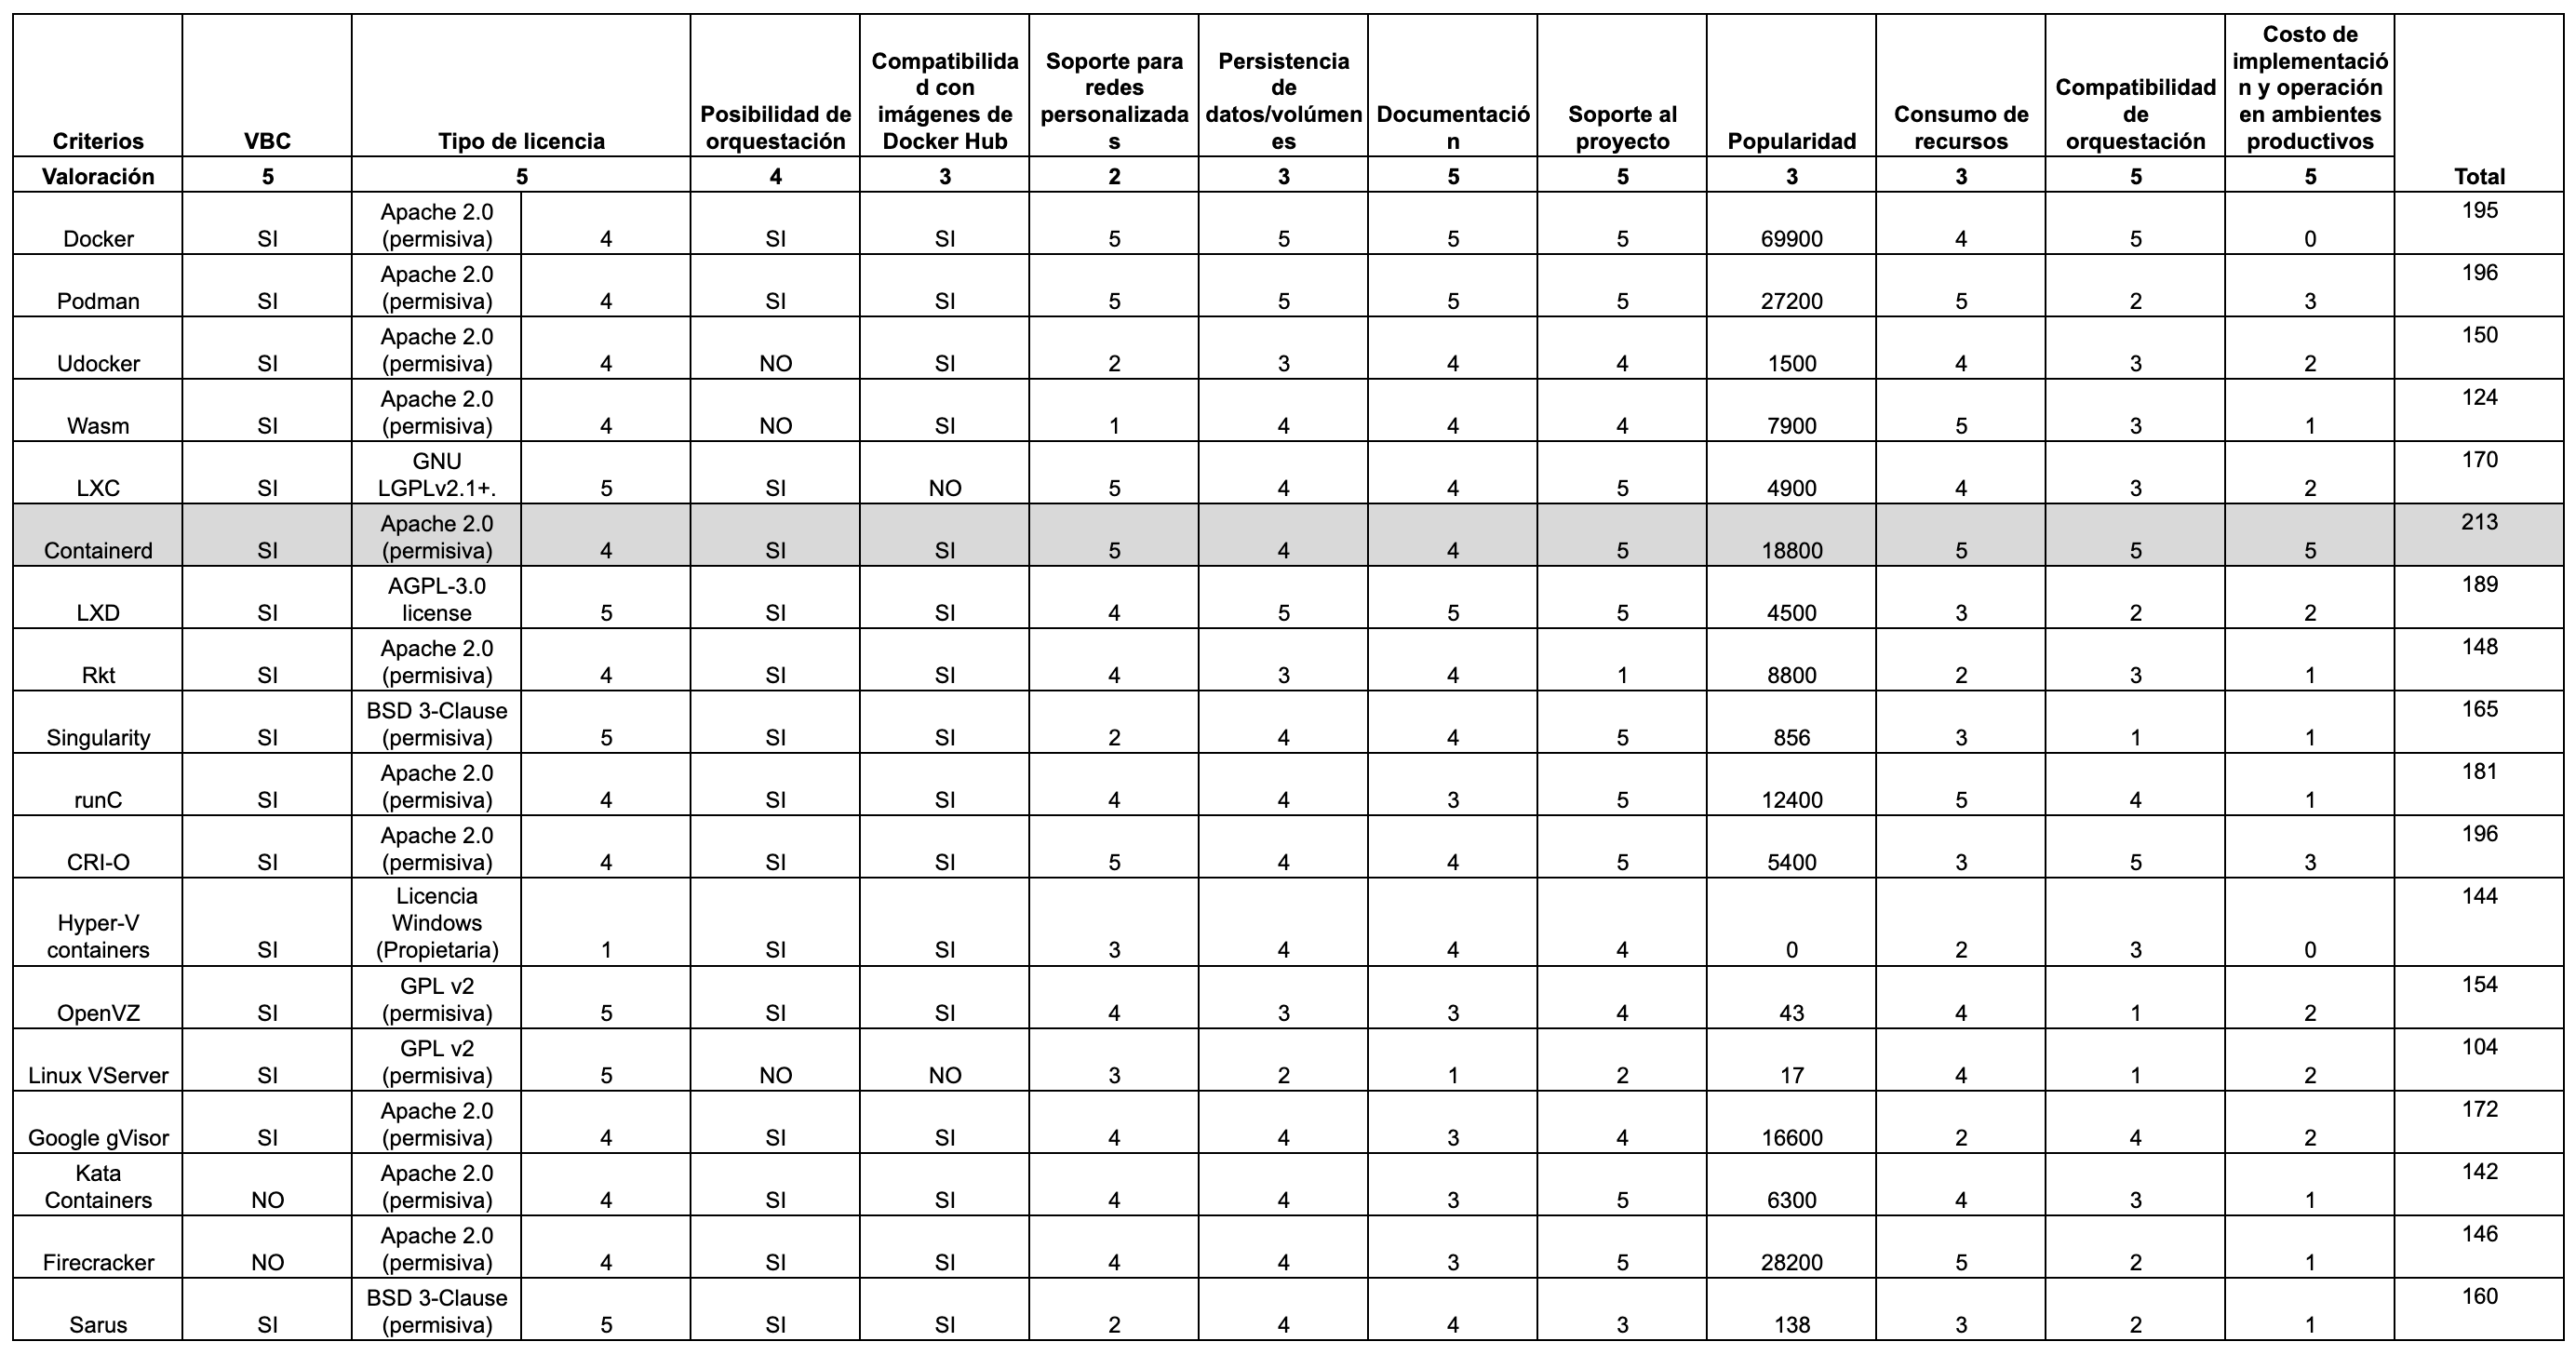
\includegraphics[width=\textwidth] {tablas-images/cp5/DAR.png}
    \caption{Análisis de Decisiones y Resolución (DAR) aplicado a la selección de VBC}\label{tab:tabla-dar}
\end{table}

\section{Criterios de evaluación}

\subsection{VBC (¿Es una tecnología basada en contenedores?)}
\noindent
Este criterio define si la tecnología analizada entra dentro de la categoría de virtualización basada en contenedores, lo cual es el punto de partida para que pueda ser considerada en el análisis. Se evalúa como Sí (SI) o No (NO).

\subsection{Tipo de licencia}
\noindent
Se analiza el tipo de licencia bajo la cual se distribuye la tecnología, ya que esto afecta su adopción en proyectos académicos o comerciales. Las licencias permisivas (como Apache 2.0 o BSD) permiten mayor libertad de uso y modificación, mientras que licencias restrictivas (como AGPL o licencias propietarias) imponen ciertas limitaciones legales o técnicas.

\subsection{Posibilidad de orquestación}\label{sec:posibilidad-orquestacion}
\noindent
Se refiere a la capacidad de la tecnología para integrarse con herramientas de orquestación como Kubernetes, Docker Swarm o Apache mesos, lo cual es clave para la gestión automatizada de contenedores a gran escala. Una mayor puntuación indica mejor compatibilidad y soporte para estas herramientas.

\subsection{Compatibilidad con imágenes de Docker Hub}
\noindent
Evalúa si la tecnología puede ejecutar imágenes obtenidas directamente desde Docker Hub, el repositorio más utilizado para contenedores. Esto facilita la reutilización de contenedores existentes y la integración con flujos de trabajo ya establecidos.

\subsection{Soporte para redes personalizadas}
\noindent
Determina si la tecnología permite la creación y gestión de redes personalizadas entre contenedores. Este aspecto es fundamental en arquitecturas distribuidas, donde la comunicación entre servicios debe configurarse de forma segura.

\subsection{Persistencia de datos / volúmenes}
\noindent
Analiza si la solución permite la persistencia de datos, es decir, que los datos generados dentro de un contenedor puedan mantenerse incluso después de reiniciarlo o eliminarlo. Esto se logra mediante el uso de volúmenes o sistemas de almacenamiento externos.

\subsection{Documentación}
\noindent
Se valora la calidad, profundidad y accesibilidad de la documentación oficial. Una buena documentación facilita el aprendizaje, la resolución de problemas y la implementación de la tecnología.

\subsection{Soporte al proyecto}
\noindent
Considera el respaldo que tiene la tecnología por parte de la comunidad, empresas o fundaciones (como CNCF o Red Hat). Esto incluye mantenimiento activo, actualizaciones regulares, y foros o canales de ayuda disponibles.

\subsection{Popularidad}
\noindent
Este criterio mide la adopción y visibilidad de la tecnología, lo cual puede reflejar su madurez, confianza del mercado y disponibilidad de talento capacitado. Se puede estimar por métricas como el número de estrellas en GitHub.

\subsection{Consumo de recursos}
\noindent
Evalúa el nivel de consumo de recursos respecto al uso de CPU, memoria y almacenamiento. Se valora según lo que mencionan las organizaciones responsables en este aspecto.

\subsection{Compatibilidad de orquestación}
\noindent
Difiere levemente del punto~\ref{sec:posibilidad-orquestacion}, ya que aquí se mide qué tan bien se integra con los orquestadores, considerando estabilidad, plugins nativos y experiencia de uso. Un puntaje alto indica integración fluida y confiable.

\subsection{Costo de implementación y operación en ambientes productivos}
\noindent
Este criterio analiza los costos asociados a poner en marcha la tecnología en un entorno real. Incluye licencias, infraestructura, tiempo de configuración y mantenimiento. Una puntuación alta significa bajo costo o costo nulo, lo cual es ideal para instituciones académicas o proyectos con presupuesto limitado.
\section{Tecnología VBC ganadora}
\noindent
Del análisis comparativo realizado, \textbf{Containerd} se posiciona como la tecnología de virtualización basada en contenedores con mejor desempeño general. Destaca por su alta compatibilidad con Docker Hub, soporte para redes y volúmenes, excelente integración con orquestadores como Kubernetes, y una licencia permisiva que facilita su adopción. Además, cuenta con una sólida documentación y un respaldo activo de la comunidad. Estas características hacen de Containerd la opción adecuada, según el análisis \DAR, para ser implementada en ambientes productivos del grupo de investigación \GRID.
\clearpage
\section{Análisis \DAR\ del motor de Kubernetes}
\noindent
El análisis presentado en la figura~\ref{tab:tabla-dar-k8s} aplica la metodología \DAR\ al proceso de selección del motor de Kubernetes más adecuado para entornos de virtualización basados en contenedores. Este enfoque estructurado permitió evaluar diversos criterios técnicos y operativos. La importancia de la elección de un motor de Kubernetes radica en su impacto directo sobre la administración de contenedores. 
\begin{table}[H]
    \centering
    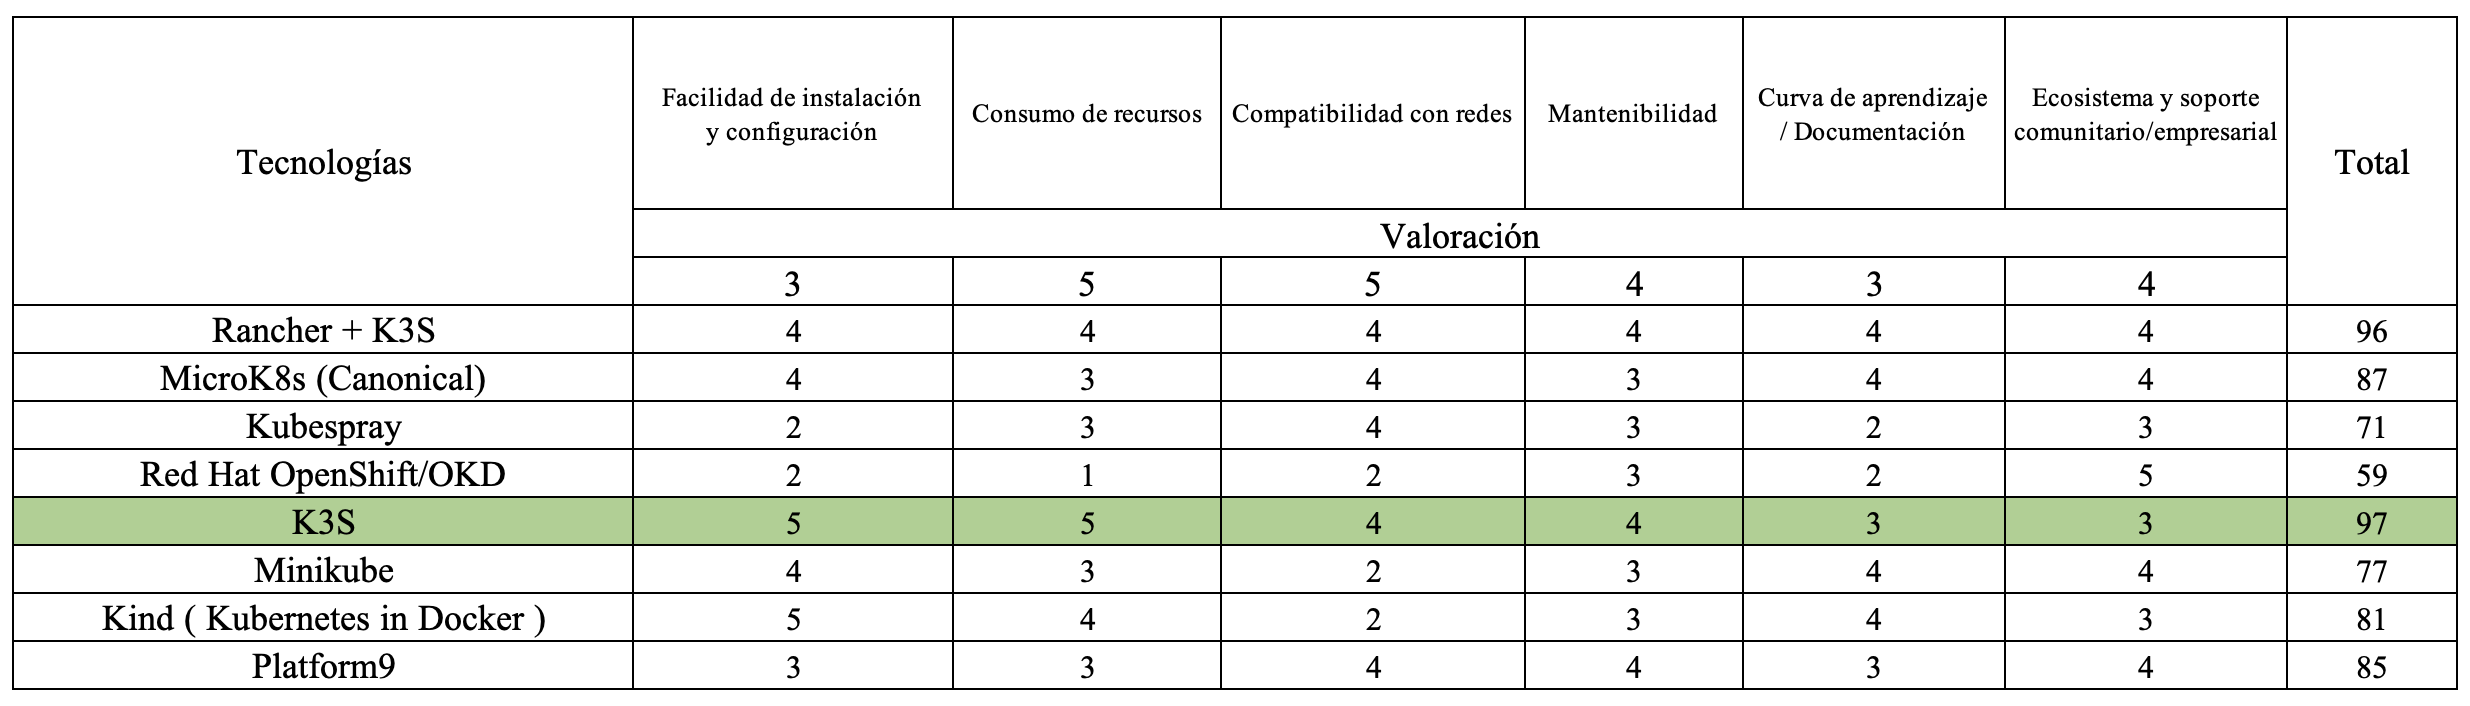
\includegraphics[width=\textwidth] {tablas-images/cp5/dar-k8s.png}
    \caption{Análisis de Decisiones y Resolución aplicado a la selección del motor de Kubernetes}\label{tab:tabla-dar}
\end{table}